\documentclass{standalone}

\usepackage{tikz}
\usetikzlibrary{calc}

\begin{document}

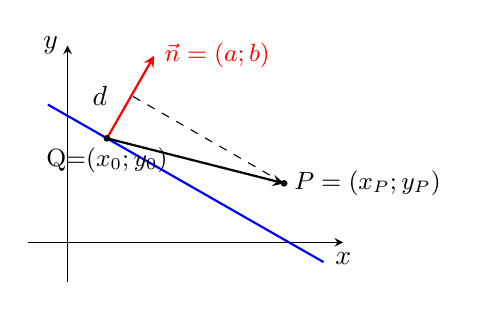
\begin{tikzpicture}[scale=1]

\draw[-stealth] (-0.5,0)--++(4,0) node[below] {$x$};
\draw[-stealth] (0,-0.5)--++(0,3) node[left] {$y$};
\draw[thick, blue] (-0.25,1.75)--(3.25,-0.25);

\draw[-stealth, thick, red] (0.5,{-0.5*4/7+45/28}) --++($0.15*(4,7)$) node[right] {\small{$\vec n = (a;b)$}};
\draw[fill=black] (0.5,{-0.5*4/7+45/28}) circle (1pt) node[below] {\small{Q=$(x_0;y_0)$}};

\node[above left] at ($(0.75,1.9)!0.5!(0.5,{-0.5*4/7+45/28})$) {$d$};

\draw[-stealth, thick, black] (0.5,{-0.5*4/7+45/28}) --(2.75,0.75) node[right] {\small{$P=(x_P;y_P)$}};
\draw[fill=black] (2.75,0.75) circle (1pt);
\draw[dashed] (2.75,0.75)--(0.75,1.9);

\end{tikzpicture}

\end{document}